\documentclass[letterpaper, 10pt]{article}
\usepackage{graphicx, xspace, subfigure,outlines,cite, framed, subfigure, hyperref,paralist,multirow,times,amsmath,
amssymb}
\usepackage[ruled,vlined]{algorithm2e}
\usepackage{xcolor}
\usepackage[footnotesize]{caption}
\pagenumbering{gobble}
%\usepackage[margin=0.5in]{geometry}

%\usepackage[small,bf]{caption}
\newcommand{\bi}{\begin{itemize}}
\newcommand{\ei}{\end{itemize}}
\newcommand{\im}{\item}
\newcommand{\eg}{{\it e.g.,}\xspace}
\newcommand{\ie}{{\it i.e.,}\xspace}
\newcommand{\secref}[1]{\S\ref{#1}}
\newcommand\eat[1]{}
\newcommand\paragraphb[1]{\vspace{0.04in}\noindent{\bf #1} }

% To make the FIXMEs go away, comment out this line...
%\newtheorem{proof}{Proof}
\newtheorem{thm}{Theorem}[section]
\newtheorem{defn}[thm]{Definition}
\newtheorem{obs}[thm]{Observation}
\newtheorem{lemma}[thm]{Lemma}
\newtheorem{theorem}{thm}[section]
\newtheorem{definition}{Definition}
\newcommand{\allnotes}[1]{}
% To make the FIXMEs go away, comment out this line...
\renewcommand{\allnotes}[1]{\textit{#1}}
\newcommand{\fixme}[1]{{\allnotes{\bf\textcolor{red}{[#1]}}}}
\newcommand{\notescott}[1]{\allnotes{\textcolor{blue}{[Scott: #1]}}}
\newcommand{\notepanda}[1]{\allnotes{\textcolor{cyan}{[Panda: #1]}}}
\newcommand{\notekaterina}[1]{\allnotes{\textcolor{green}{[Panda: #1]}}}
\def\squarebox#1{\hbox to #1{\hfill\vbox to #1{\vfill}}}

\usepackage{framed}
\colorlet{shadecolor}{gray!25}   % you may try 'blue' here
\renewenvironment{leftbar}{%
  \def\FrameCommand{\textcolor{shadecolor}{\vrule width 3pt} \hspace{10pt}}%
  \MakeFramed {\advance\hsize-\width \FrameRestore}\small}%
{\normalsize \endMakeFramed}

\newcommand{\katnote}[1]{\allnotes{[\textcolor{blue}{\textit{Kat: #1}}]}}


%\title{Model Checking for Dynamic Datapaths}
%\author{Paper \#82, 14 pages}
\title{Notes on Static Routing}
\date{}

%\special{papersize=8.5in,11in}
%\setlength{\pdfpageheight}{\paperheight}
%\setlength{\pdfpagewidth}{\paperwidth}

\begin{document}
\maketitle
\thispagestyle{empty}
\begin{figure}[ht]
    \begin{center}
        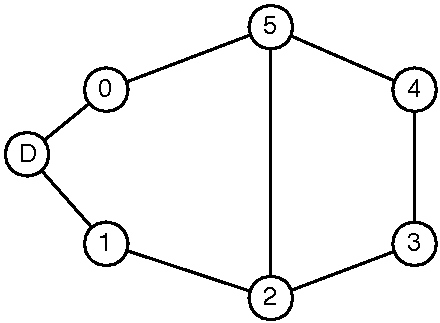
\includegraphics[width=0.5\textwidth]{topo.pdf}
        \caption{Example topology}
        \label{fig:topology}
    \end{center}
\end{figure}

We only talk about a single destination. In Figure~\ref{fig:topology} this destination is depicted by $D$.

Some items based on what we talked about today:
\begin{itemize}
    \item Each node has a routing table of size $k$ where $k$ is the degree of the node.
    \item The routing table chooses $k$ of ${k \choose 2}$ possible options. Actually we choose from among $k^2$ choices
        (we allow loops). 
    \item The question to consider here is do we get perfect resilience.
\end{itemize}

Just so we are on the same page, the model is the following:
\begin{itemize}
    \item We are using per-destination routing tables based on the input port (link).
    \item The nodes are memoryless.
    \item If node $N$ sends a packet to node $M$ after the $N$---$M$ link has failed the packet appears at node $N$ as
        if it was sent by $M$. In particular this means that in Figure~\ref{fig:topology} if the $5$---$0$ link was
        failed and node $5$ send a packet to $0$ then we pretend node $5$ receives the same packet from node $0$, \ie we
        look at the table entry for $0$.
\end{itemize}

Some observations and hypothesis:
\begin{itemize}
    \item For maximal resilience a node should use every link it has; if this is not the case just fail all but that
        link.
    \item While we allow nodes to send traffic back on the link they received it this seems suboptimal given that this
        make it super simple to make a loop appear.
    \item \textbf{Hypothesis}: Based on above a maximally resilient routing table at a node should be a permutation of all of the links.
\end{itemize}

\begin{figure*}[h]
\subfigure[Routing table for Node 5.]{
    \begin{tabular}{|c|c|}
            \hline
            Src & NHop\\
            \hline
            \hline
            4 & 0\\
            \hline
            0 & 2\\
            \hline
            2 & 4\\
            \hline
    \end{tabular}
    \label{tab:n5route}
}
\hspace{0.2in}
\subfigure[Routing table for Node 2.]{
    \begin{tabular}{|c|c|}
            \hline
            Src & NHop\\
            \hline
            \hline
            5 & 1\\
            \hline
            1 & 3\\
            \hline
            3 & 5\\
            \hline
    \end{tabular}
    \label{tab:n2route}
}
\end{figure*}

If the hypothesis is correct then case Figure~\ref{fig:topology} is not maximally resilient. In particular the problem
here is with the interplay of permutation for node $5$ and node $2$. As en example consider the permuataion  $4-0-2$ 
(\ie the routing table in Table~\ref{tab:n5route}) for node $5$. In this case to avoid loops $2$ must choose to send all
packets from $5$ to node $1$. So the only permutations left is $5-1-3$ resulting in the routing table~\ref{tab:n2route}.
At this point given any strategy by $3$ or $4$ one can find failures that induce a loop: 

If $3$ sends traffic from $4$ to $2$ then just fail $2$--$1$ and $4$--$5$ to induce a loop despite connectivity. So
clearly perfect connectivity is not possible. 

Now the questions:
\begin{itemize}
    \item For your counting argument in this setting would you say there are more than $3$ paths through $5$ and hence
        the problem? (I count $5$---$0$, $5$---$2$---$1$, $5$---$4$---$3$---$2$---$1$ which is why I am not sure how to
        play our the counting argument. I guess this is more obvious for $4$ which has $4$---$5$---$0$,
        $4$---$3$---$2$---$1$, $4$---$5$---$2$---$1$, $4$---$3$---$2$---$5$---$0$ and only $2$ possible actions, but the
        concern there is that I it feels like we should somehow be counting choices along the path somehow).
    \item Did I miss something that you had in your model?
\end{itemize}

\end{document}
